\documentclass{article}
\usepackage[utf8]{inputenc}
\usepackage[margin=1in]{geometry}
\usepackage{mathptmx}
\usepackage{subcaption}
\setlength{\parindent}{0em}
\setlength{\parskip}{0.5em}


\title{Assignment 2 - CTA200H}
\author{Mukesh Taank (mtaank)}
\date{May 8, 2020}

\usepackage{natbib}
\usepackage{graphicx}

\begin{document}

\maketitle

\section*{Question 1}

This question deals with looking at plotting points on the complex plane. 
We are given our initial starting position $z_0$ to be 0.
Then we are told to iterate according to the equation $z_{i + 1} = z_i^2 + c$.
We are also told to focus the area of the plane: $-2 < x < 2$ and $-2 < y < 2$.
I chose a few random points, $c$ and plotted the iterations of $z$.
The following plot shows the iterations of the chosen points using the initial start at zero.

\begin{figure}[!ht]
    \centering
    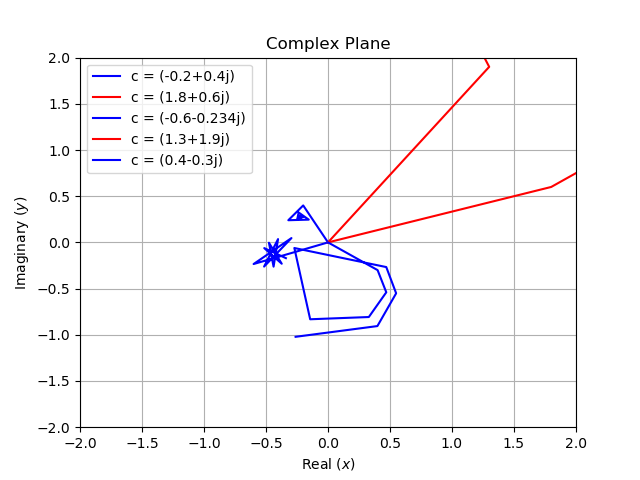
\includegraphics[scale=0.9]{Q1_plot1.png}
    \caption{Plot of the complex plane, showing the iterations of $z_i$ with different selection of C.}
    \label{fig:Q1_plot1.png}
\end{figure}

The red graphs represent the points that cause the iteration of $z_i$ to blow up to plus/minus infinity. 
The blue graphs represent the points that cause the iterations of $z_i$ to be contained in the boundaries.

One thing I noticed when plotting this is that the iterations will make $z_i$ either diverge or stay bounded depending on the modulus of the complex number, $c$.
I have printed the moduli of the complex numbers I chose to plot, seen in figure two.

\begin{figure}[!ht]
    \centering
    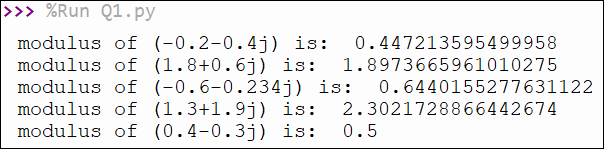
\includegraphics[scale=0.75]{Q1_pic.png}
    \caption{Output of the code $Q1.py$ showing the modulus of the various complex numbers, c, shown in the above figure.}
    \label{fig:Q1_pic.png}
\end{figure}

What we observe is that when the modulus of the chosen complex number is > 1, iterations of the equation: $z_{i + 1} = z_i^2 + c$ tend to diverge to infinity in either the +/- direction. If the modulus of the complex number is < 1, the iterations of the equation stay within the bounds of the plane.

We can also look at the iterations of the above equation with a colourscale. Figure 3 shows the iterations using different complex numbers.
For the complex numbers that cause the iterations to diverge, within the 2x2 plane, we will not see all the points.
For the complex numbers that keep the iterations bounded in the 2x2 plane, we will see all the points and all colours of the points.

\begin{figure}[!ht]
    \centering
    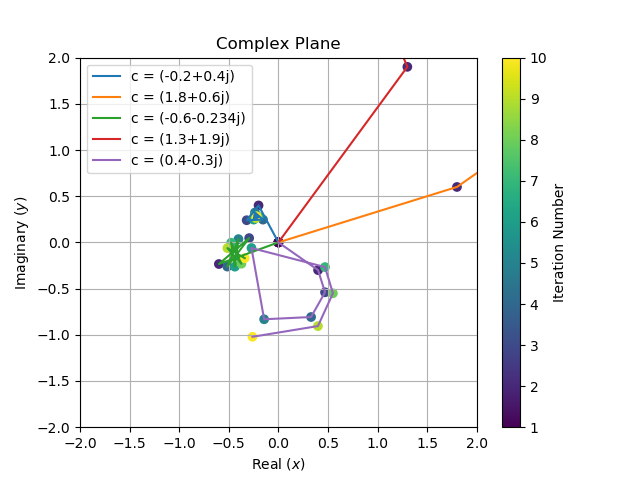
\includegraphics[scale=0.9]{Q1_plot2.png}
    \caption{Plot of the complex plane, showing the iterations of the equation above using a colour scale to represent the current iteration.}
    \label{fig:Q1_plot2.png}
\end{figure}

From this, we can see that the red and orange plots, which have modulus > 1, diverge to infinity and we cannot see all the colours along the colour bar. On the other hand, for the purple, green and blue plots, we see all the colours on the colour bar.


\section*{Question 2}

This question deals with looking at the SIR model, which is a simple mathematical model of disease spread in a population. 
We are given a set of ordinary differential equations by which this spread is modelled by. 
Using the given initial conditions and differential equations, I was able to use an ODE integrator to solve for the $S$, $I$ and $R$ functions to get their relations with respect to time.
One thing that needed to be done first was to find realistic values for the parameters $\beta$ and $\gamma$. 

$\beta$ represents the rate of the spread of infection per contact between infected and non-infected per unit time.
$\gamma$ represents the rate at which the infected recover per unit time.

From this, I can assume reasonable values for $\beta$ and $\gamma$, which are between 0 and 1. 
If we assume beta is, for example, 0.5, then this is saying that the disease is spread through 1 meeting between the infected and non-infected every 2 days. 
If we assume gamma is, for example, 0.5, then this is saying one person will recover every 2 days.

\bigskip
To approach this problem, I used the built-in function in SciPy: scipy.integrate.odeint() in order to solve the set of differential equations.
When I solved the set of ODEs and finally got my solution functions, I then plotted them onto one graph using varying values for $\gamma$ and $\gamma$ to see how the curves would change with respect to these parameters.
The following figures show the plots of $S(t)$, $I(t)$ and $R(t)$ with different values of $\beta$ and $\gamma$.

\begin{figure}[!ht]
  \centering
  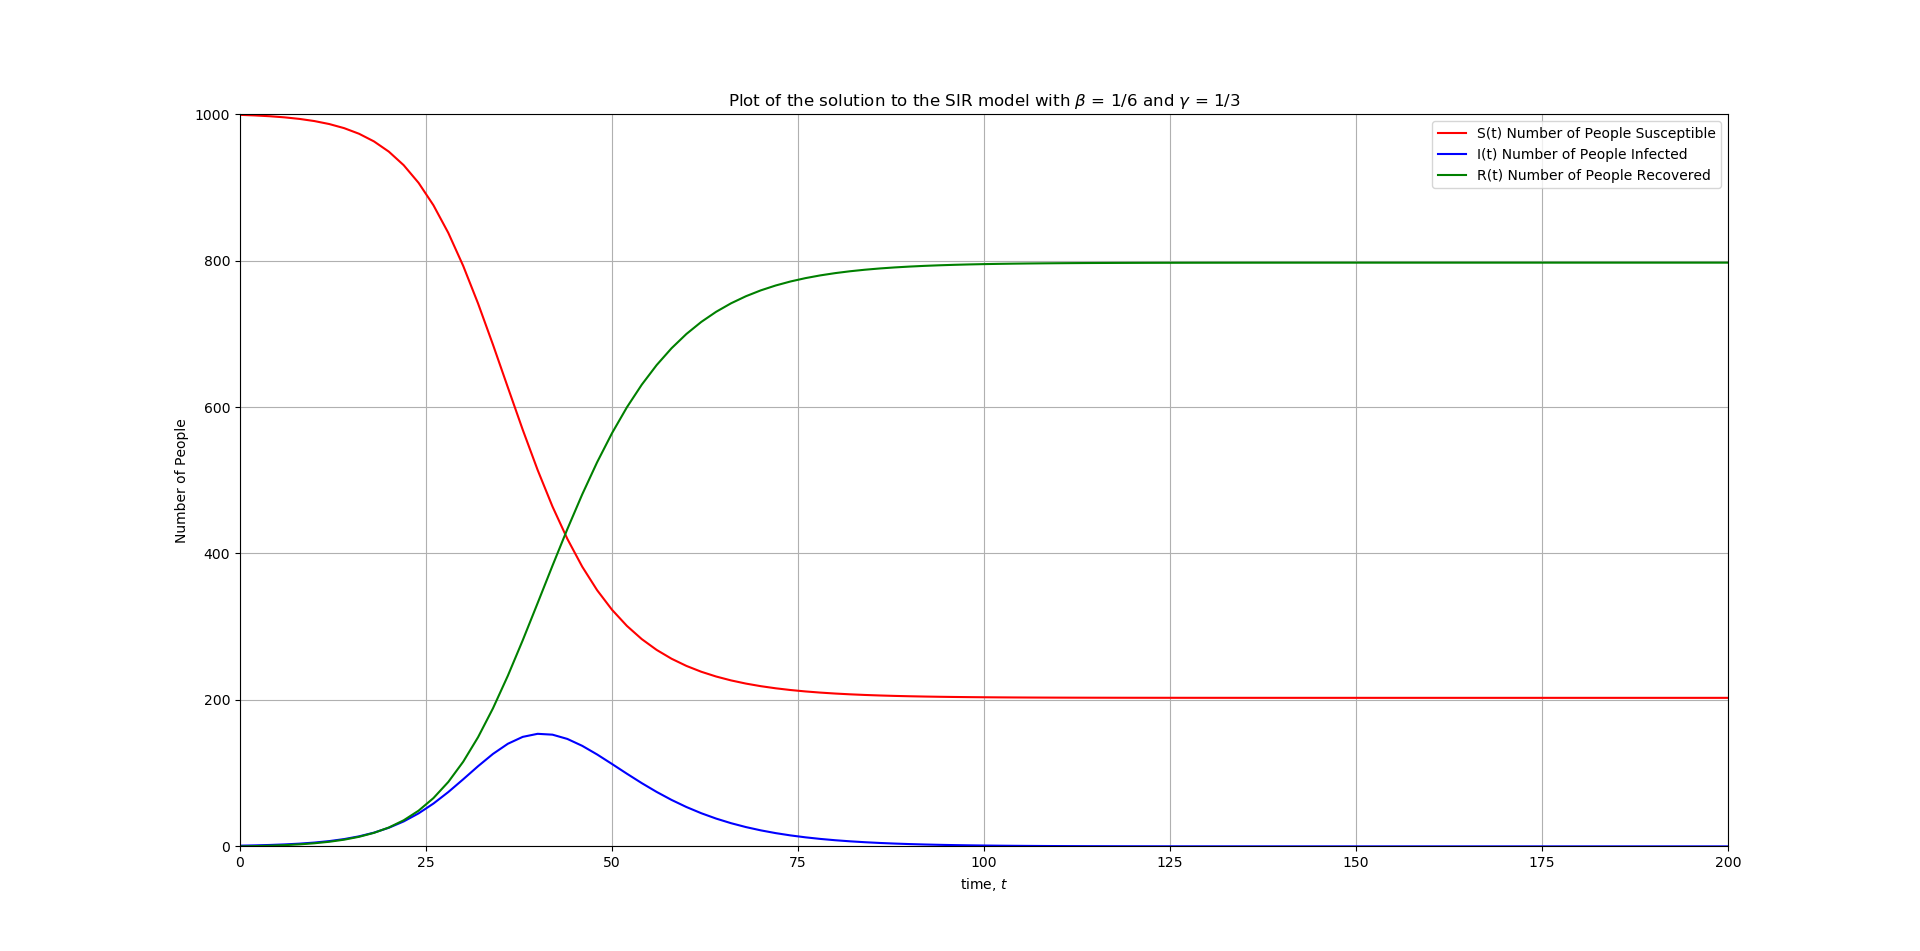
\includegraphics[width=1\linewidth]{Q2_plot1.png}
  \caption{Plot of the solution functions; $S(t)$, $I(t)$ and $R(t)$ \\ over time, with $\beta$ = 1/6 and $\gamma$ = 1/3.}
  \label{fig:Q2_plot1.png}
\end{figure}

\begin{figure}[!hp]
  \centering
  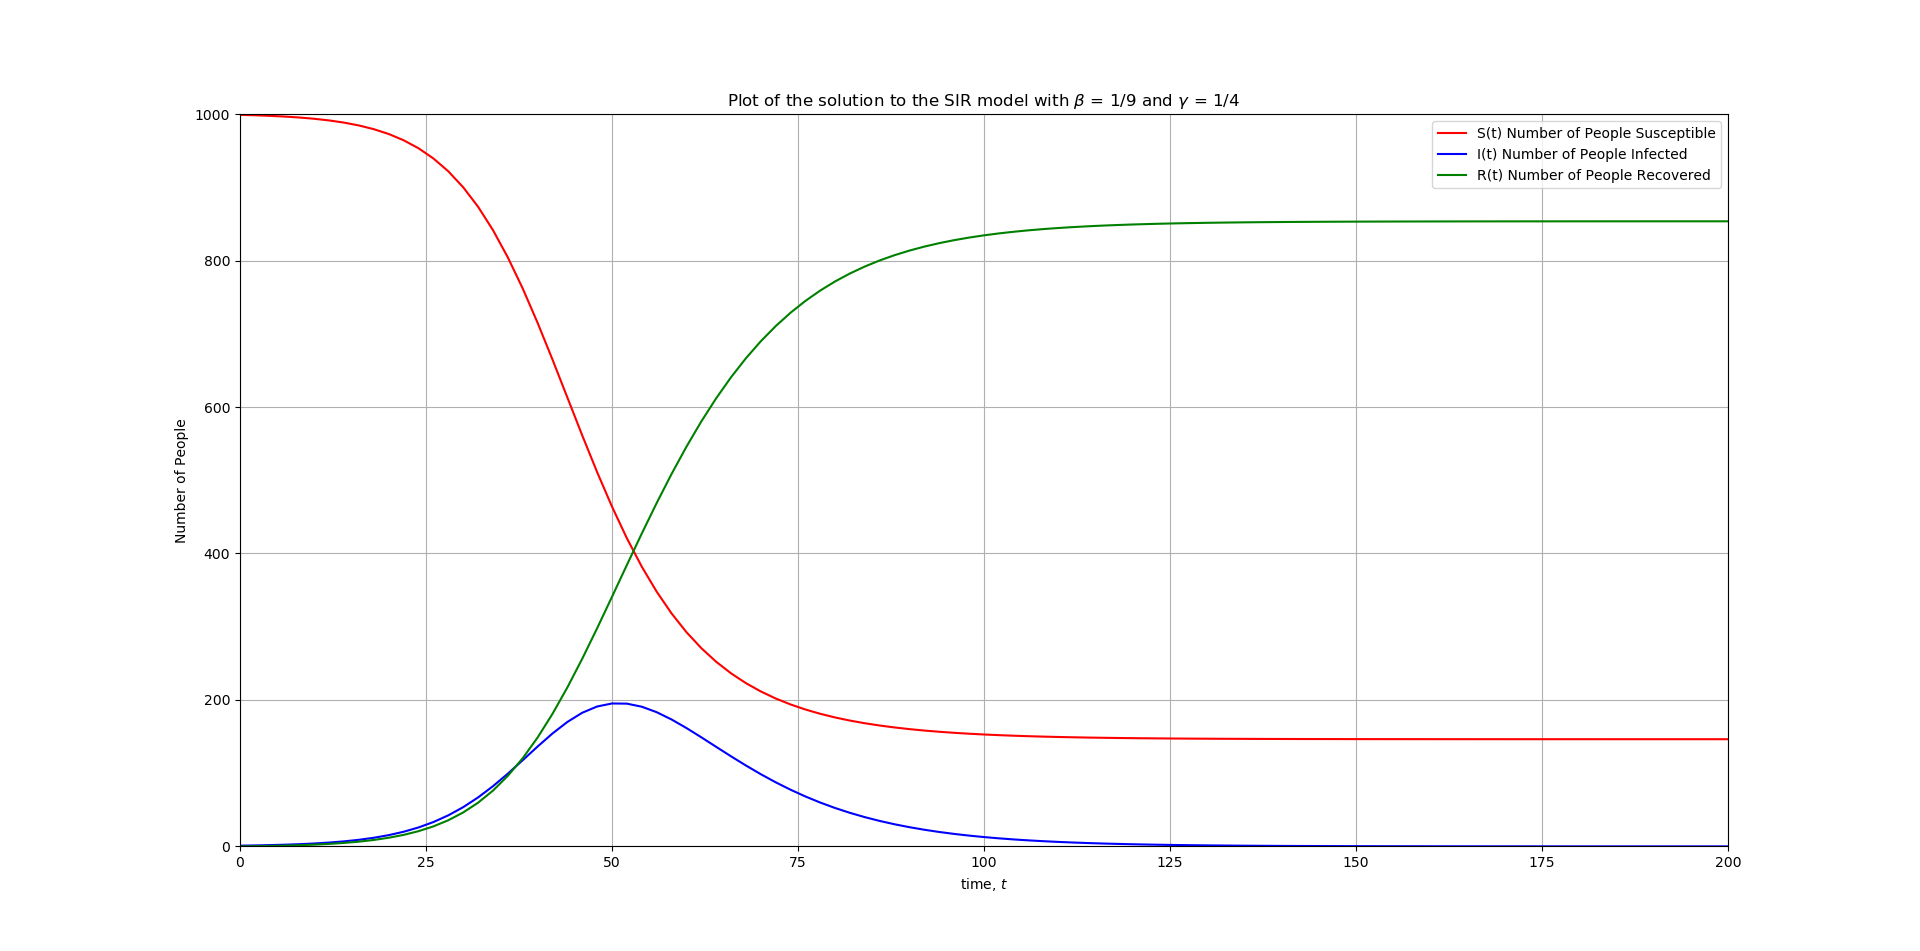
\includegraphics[width=1\linewidth]{Q2_plot2.png}
  \caption{Plot of the solution functions; $S(t)$, $I(t)$ and $R(t)$ \\ over time, with $\beta$ = 1/9 and $\gamma$ = 1/4.}
  \label{fig:Q2_plot2.png}
\end{figure}

\begin{figure}[!hp]
  \centering
  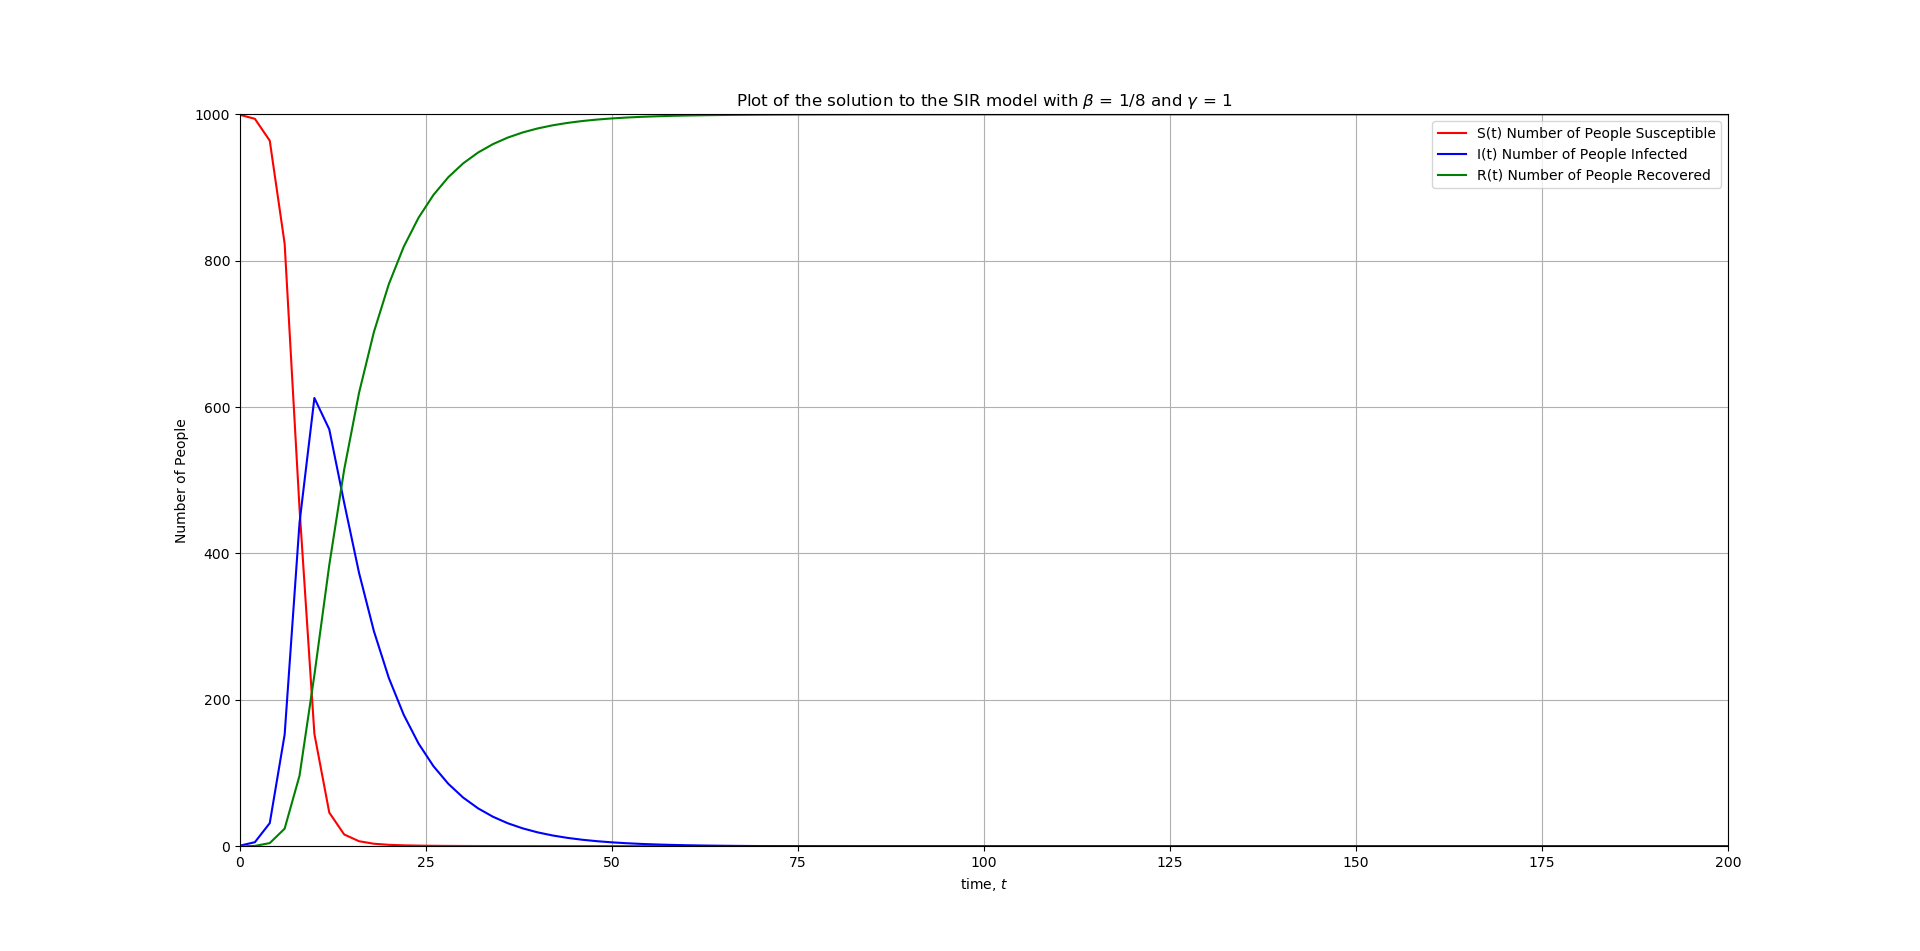
\includegraphics[width=1\linewidth]{Q2_plot3.png}
  \caption{Plot of the solution functions; $S(t)$, $I(t)$ and $R(t)$ \\ over time, with $\beta$ = 1/8 and $\gamma$ = 1.}
  \label{fig:Q2_plot3.png}
\end{figure}

\begin{figure}[!hp]
  \centering
  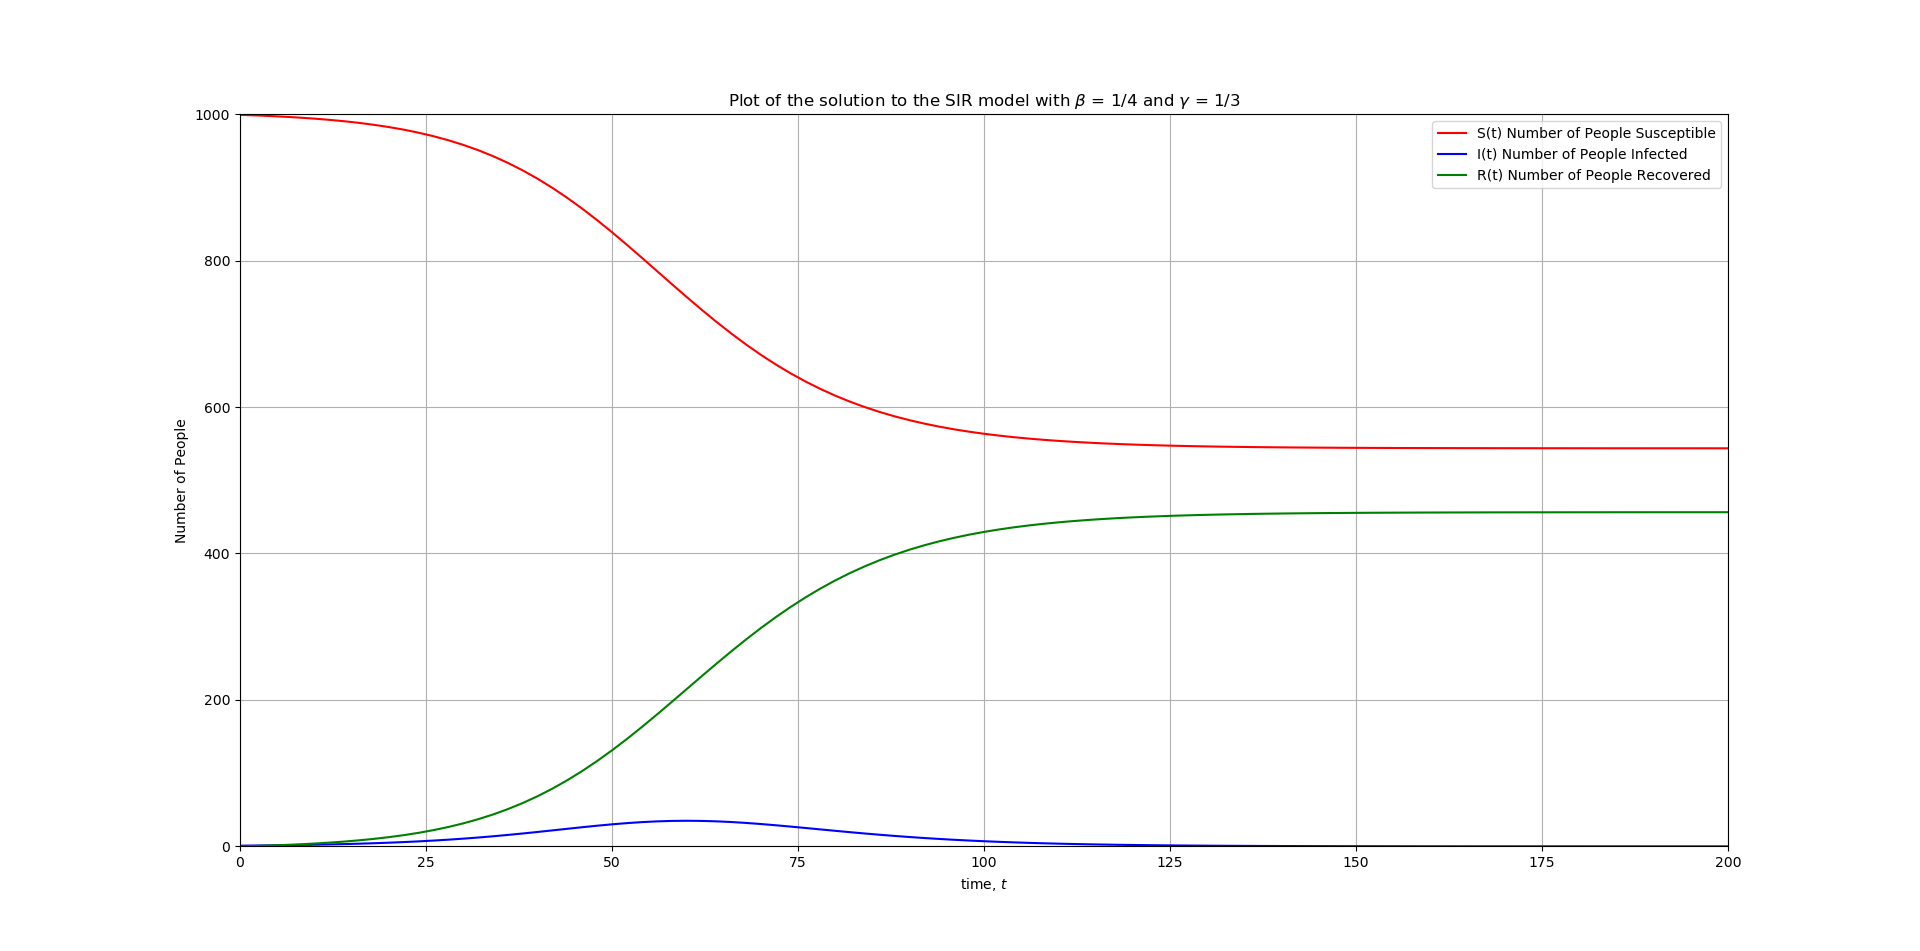
\includegraphics[width=1\linewidth]{Q2_plot4.png}
  \caption{Plot of the solution functions; $S(t)$, $I(t)$ and $R(t)$ \\ over time, with $\beta$ = 1/4 and $\gamma$ = 1/3.}
  \label{fig:Q2_plot4.png}
\end{figure}
\bigskip
\bigskip

Looking at Figure 4, we have a $\beta$ value of 1/6 and a $\gamma$ value of 1/3. 
So in this case, $\beta$ $<$ $\gamma$.
From this relation, we see that the peak of the number of people infected is about 170, and happens around day number 43.
The number of people susceptible and number of people recovered actually equal at  about day 42.
In this case, the peak number of infected people is relatively low.
\bigskip

In Figure 5, we have a $\beta$ value of 1/9 and a $\gamma$ value of 1/4. 
So in this case, $\beta$ $<$ $\gamma$.
From this relation, we see that the peak of the number of people infected is about 200, and happens around day number 50.
The number of people susceptible and number of people recovered actually equal at  about day 42.
This plot is very similar to figure 4, as the general shape of the curves is consistent.
In this case, the peak number of people infected is relatively low.
\bigskip

In Figure 6 below, we have a $\beta$ value of 1/8 and a $\gamma$ value of 1. 
So in this case, $\beta$ $<<$ $\gamma$.
From this relation, we see that the peak of the number of people infected is about 600, and happens around day number 12.
The number of people that are susceptible to the virus decreases very fast, starts at 1000 and reaches zero in about 18 days.
This also means that the number of people that were infected did make a recovery since the recovery curve reaches the maximum of 1000.
So with this combination of $\beta$ and $\gamma$, we see a relatively high peak that occurs very fast.
Since the peak of the number of people infected happened very early, the number of people infected dropped off quickly and eventually reached zero after about 60 days.
Also, everyone is healthy from the virus/disease after the same 60 days and no one is susceptible any more.
This plot is very similar to figure 4, as the general shape of the curves is consistent.
In this case, the peak number of people infected is relatively high.
\bigskip

In Figure 7, we have a $\beta$ value of 1/4 and a $\gamma$ value of 1/3. 
So in this case, $\beta$ $\approx$ $\gamma$.
From this relation, we see that the peak of the number of people infected is only about 30 people, and happens around day number 60.
So with this combination of $\beta$ and $\gamma$, we see a very low peak, indicating that the virus is not spreading very fast at all.
After around 110 days, there are no longer any people infected.One thing that is different in this graph compared to the others is that the number of people susceptible and the number of people the recover, are never equal. Since not many people get infected in the first place, the number of susceptible people goes down relatively fast and the opposite for the number of people recovered, it goes up relatively quickly.
This plot is very similar to figure 4, as the general shape of the curves is consistent.
In this case, the peak number of people infected is relatively high.

\bigskip
From analyzing the different variations of $\beta$ and $\gamma$, we can see how likely a virus/disease is to spread among a given population given the amount of times people are in contact with each other (which comes from the two parameters).


\end{document}